\subsubsection{Klassebeskrivelser}

Herunder ses en  beskrivelse af samtlige klasser i business logic layer. Beskrivelsen vil fremgå som \textit{klassenavn"} efterfulgt af en kort beskrivelse af klassens ansvar og funktionalitet.\\\\


\textbf{Brains} namespacet indeholder generel businesslogik for at kunne udføre handlinger, så som at oprette kommandoer, parse objekter til XMl mv. Den benytter sig meget af det delte bibliotek \gls{SL}.\\

\paragraph{ViewModels} namespacet indeholder viewmodels til alle views. Viewmodels indeholder den data som præsentationslaget binder til. Dette indebærer kommandoer til knapper, samt properties som skal bruges af viewet.\\

\textbf{MainWindowViewModel}\\
Denne viewmodel hører til MainWindow, som er hovedvinduet i \gls{AS}. Denne viewmodel indeholder alle produktkategorier, som har lister med produkter. Derudover er der kommandoer til at åbne alle andre vinduer i systemet. Denne viewmodel har subscribed på alle andre viewmodels "Loaded" events. Se nærmere omkring disse under afsnit \ref{WindowLoadedEvents_Beskrivelse}, side \pageref{WindowLoadedEvents_Beskrivelse}.
\begin{figure}[H]
	\centering
	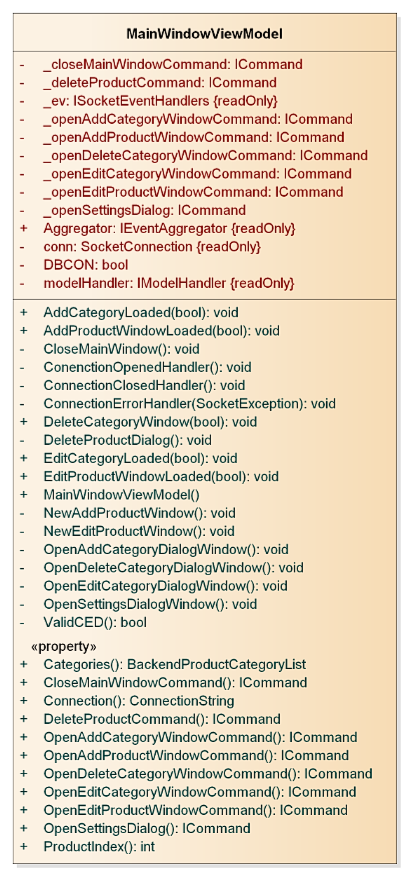
\includegraphics[width=0.5\textwidth]{Systemdesign/backend/klassebeskrivelser/Images/MainWindowVM}
	\caption{MainWindowViewModel}
	\label{fig:MainWindowViewModel}
\end{figure}
\bigskip

\textbf{AddProductViewModel}\\
Denne viewmodel hører til AddProductWindow og indeholder kommandoer og data der skal bruge for at oprette et nyt produkt. Dette indebærer bl.a. listen af produktkategorier, samt kommandoer til at oprette og annullere oprettelsen.
\begin{figure}[H]
	\centering
	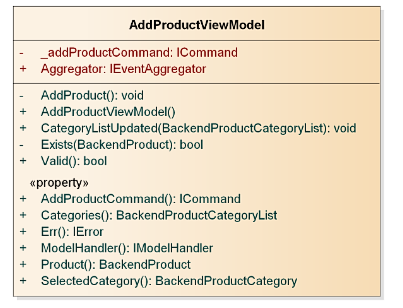
\includegraphics[width=0.5\textwidth]{Systemdesign/backend/klassebeskrivelser/Images/AddProductVM}
	\caption{AddProductViewModel}
	\label{fig:AddProductViewModel}
\end{figure}
\bigskip

\textbf{EditProductViewModel}\\
Denne viewmodel hører til EditProductViewModel og indeholder kommandoer og data der skal bruges for at redigere et eksisterende produkt.
\begin{figure}[H]
	\centering
	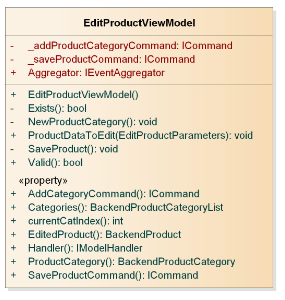
\includegraphics[width=0.5\textwidth]{Systemdesign/backend/klassebeskrivelser/Images/EditProductVM}
	\caption{EditProductViewModel}
	\label{fig:EditProductViewModel}
\end{figure}
\bigskip

\textbf{AddCategoryViewModel}\\
Denne viewmodel hører til AddCategoryWindow og indeholder kommandoer og data der skal bruge for at oprette en ny produktkategori.
\begin{figure}[H]
	\centering
	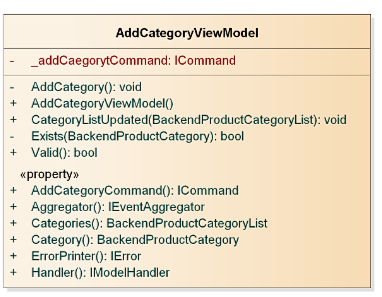
\includegraphics[width=0.5\textwidth]{Systemdesign/backend/klassebeskrivelser/Images/AddCategoryVM}
	\caption{AddCategoryViewModel}
	\label{fig:AddCategoryViewModel}
\end{figure}
\bigskip

\textbf{EditCategoryViewModel}\\
Denne viewmodel hører til EditCategoryWindow og indeholder kommandoer og data der skal bruge for at redigere en produktkategori.
\begin{figure}[H]
	\centering
	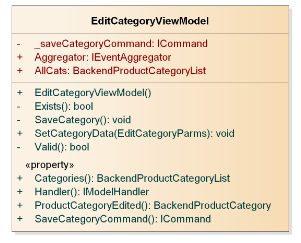
\includegraphics[width=0.5\textwidth]{Systemdesign/backend/klassebeskrivelser/Images/EditCategoryVM}
	\caption{EditCategoryViewModel}
	\label{fig:EditCategoryViewModel}
\end{figure}
\bigskip

\textbf{DeleteCategoryViewModel}\\
Denne viewmodel hører til DeleteCategoryWindow og indeholder kommandoer og data der skal bruge for at slette en produktkategori.
\begin{figure}[H]
	\centering
	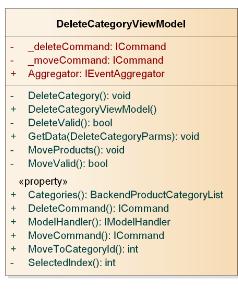
\includegraphics[width=0.5\textwidth]{Systemdesign/backend/klassebeskrivelser/Images/DeleteCategoryVM}
	\caption{DeleteCategoryViewModel}
	\label{fig:DeleteCategoryViewModel}
\end{figure}
\bigskip

\paragraph{Brains} namespacet indeholder generel businesslogik for at kunne udføre handlinger, så som at oprette kommandoer, parse objekter til XMl mv. Den benytter sig meget af det delte bibliotek \gls{SL}.\\

\textbf{Error}\\
Errorklassen er en fejlbeskedprinter, som kan printe en besked på skærmen, eksempelvis ved fejl eller notifikationer.
\begin{figure}[!h]
    \centering
    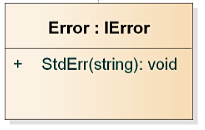
\includegraphics[width=0.2\textwidth]{Systemdesign/backend/klassebeskrivelser/Images/Error.png}
    \caption{Error}
    \label{fig:error}
\end{figure}
 \bigskip 
 
 
 
 
 
 
 


\textbf{ModelHandler}\\
ModelHandlerens ansvar er at lave den kommando der skal sendes til \gls{CS}. Denne kommando kan være til for eksempelvis at oprette eller nedlægge et produkt. Denne klasse er desuden den klasse, som kalder klienten til at sende den netop oprettede kommando. 
\begin{center}
\begin{figure}[!h]
    \centering
    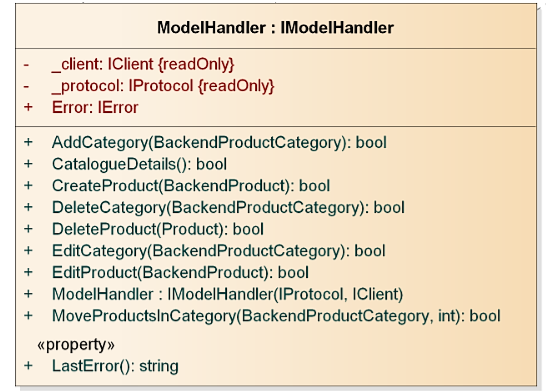
\includegraphics[width=0.45\textwidth]{Systemdesign/backend/klassebeskrivelser/Images/ModelHandler.png}
    \caption{ModelHandler}
    \label{fig:modelhandlerreal}
\end{figure}
\end{center}
\label{Modelhandler_Beskrivelse}
 \bigskip
 
 
 
 
 

\textbf{PrjProtokol}\\
PrjProtokol har til ansvar at lave kald til \gls{SL} og dens protokol.Den sørger udelukkende for at få lavet de rigtige kald, for at få et eventuelt objekt parset om til en XML-streng, igen. \bigskip
\begin{center}
\begin{figure}[!h]
    \centering
    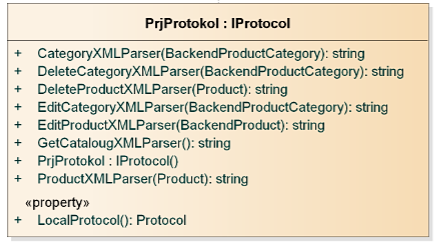
\includegraphics[width=0.45\textwidth]{Systemdesign/backend/klassebeskrivelser/Images/PrjProtokol.png}
    \caption{ModelHandler}
    \label{fig:prjprotko}
\end{figure}
\end{center}
\label{PrjProtokol_Beskrivelse}
 \bigskip
 




\bigskip
\bigskip




\textbf{Events} namespacet indeholder klasser, som fungerer som events, til brug i kommunikation mellem viewmodels. Der vil i dette afsnit beskrives flere klasser i en beskrivelse, da de er så ens som de er. Der er desuden dataobjekter i dette namespace, til brug i sammenhæng med events.\\
\bigskip

\textbf{EditProductParameters, EditCategoryParms, DeleteCategoryParms}\\
Et objekt indeholdende data der bliver brugt i en anden viewmodel, når NewEditProductData eventet raises. Dette bruges da kun én parameter kan bruges i disse events. Kommunikation mellem viewmodels er beskrevet nærmere på side \pageref{viewcomm}. \bigskip
\begin{center}
\begin{figure}[!h]
    \centering
    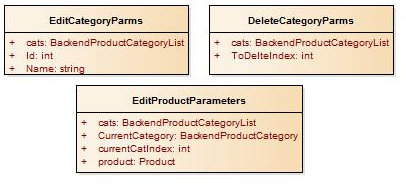
\includegraphics[width=0.50\textwidth]{Systemdesign/backend/klassebeskrivelser/Images/Parms.png}
    \caption{Paramtereklasser}
    \label{fig:EditProductParameters}
\end{figure}
\end{center}
\label{EditProductParameters_Beskrivelse}
 \bigskip 




\textbf{CategoryListUpdated, NewEditProductData, NewEditCategoryData, NewDeleteCategoryData}
Disse arver ale sammen fra PubSubEvent\footnote{En eventtype som bruges i PRISM ~\cite{PRISM}}. Disse events raises når et vindue med en anden viewmodel er loaded, og der ønskes at dele data mellem disse viewmodels. Kommunikation mellem viewmodels er beskrevet nærmere på side \pageref{viewcomm}.  \bigskip
\begin{center}
\begin{figure}[!h]
    \centering
    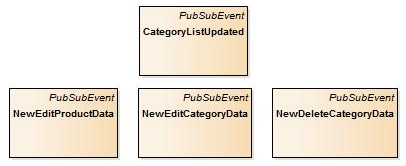
\includegraphics[width=0.50\textwidth]{Systemdesign/backend/klassebeskrivelser/Images/Events1.png}
    \caption{Events}
    \label{fig:CategoryListUpdated}
\end{figure}
\end{center}
\label{CategoryListUpdated_Beskrivelse}
 \bigskip 



\label{WindowLoadedEvents_Beskrivelse}
\textbf{AddProductWindowLoaded, DeleteCategoryWindowLoaded, EditCategoryWindowLoaded, AddCategoryWindowLoaded, EditProductWindowLoaded}
Disse klasser arver ale sammen fra PubSubEvent\footnote{En eventtype som bruges i PRISM ~\cite{PRISM}}. De fungerer således som et event de raises, når et vindue loades, således at der kan deles data. Kommunikation mellem viewmodels er beskrevet nærmere på side \pageref{viewcomm}. \bigskip
\begin{center}
\begin{figure}[!h]
    \centering
    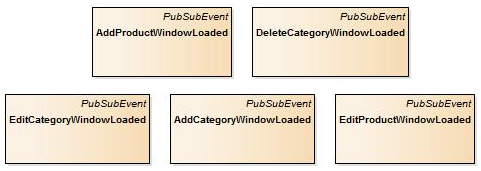
\includegraphics[width=0.50\textwidth]{Systemdesign/backend/klassebeskrivelser/Images/Events2.png}
    \caption{Events}
    \label{fig:AddProductWindowLoaded}
\end{figure}
\end{center}
\label{AddProductWindowLoaded_Beskrivelse}
 \bigskip 


\bigskip
\bigskip

\textbf{SocketEvents} namespacet indeholder klasser til brug i forbindelse med events raised fra \gls{SL}.\\
\bigskip

\textbf{SocketEventHandlers}\\
Denne klasse indeholder alle eventhandlere som bruges, når der bliver raised et event fra \gls{SL}'s sockets. Dette kunne eksempelvis være et event der fortæller at produktlisten er opdateret eller lignende. Den har desuden subscribemetoder, som bruges til at subscribe på disse events.
\begin{center}
\begin{figure}[!h]
    \centering
    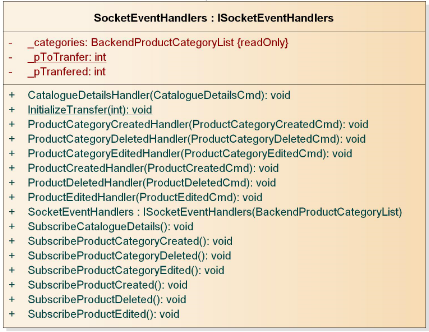
\includegraphics[width=0.50\textwidth]{Systemdesign/backend/klassebeskrivelser/Images/SocketEvents.png}
    \caption{SocketEventHandlers}
    \label{fig:SocketEventHandlers}
\end{figure}
\end{center}
\label{SocketEventHandlerBeskrivelse}
 \bigskip 
 
 
\textbf{SingleEventAggregator}\\
Denne klasse indeholder en EventAggregator fra PRISM~\cite{PRISM}, som man håndterer alle events, publishers og subscribers. Denne er implementeret som en singleton, således alle der bruger denne, bruger den samme.
\begin{center}
\begin{figure}[!h]
    \centering
    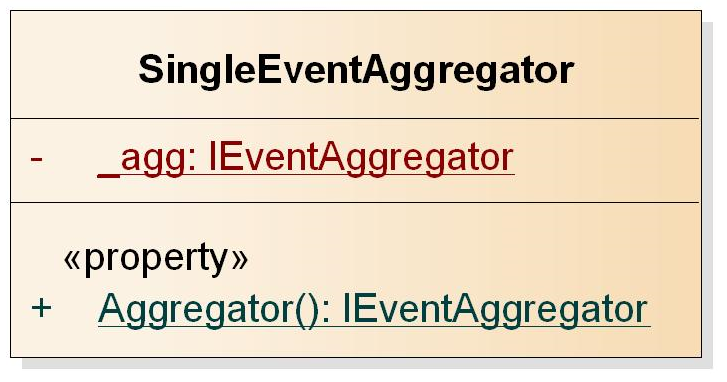
\includegraphics[width=0.30\textwidth]{Systemdesign/backend/klassebeskrivelser/Images/agg.png}
    \caption{SingleEventAggregator}
    \label{fig:SingleEventAggregator}
\end{figure}
\end{center}
\label{SingleEventAggregator_Beskrivelse}
 \bigskip 

\bigskip
\bigskip

\textbf{Datamodels} namespacet indeholder alle datamodeller. Det er disse datamodeller hele systemet benytter.\\
\bigskip

\textbf{BackendProductCategoryList}\\
Denne klasse indeholder en liste af kategorier. Det er denne datatype som indeholder al data fra \gls{DB} , når det hentes ned fra \gls{CS}. Denne klasse arver fra en anden klasse, ASyncObservableCollection, som er skrevet af Thomas Levesque~\cite{ASYNC}. Dette har været nødvendigt, da der i nogle tilfælde ville være flere tråde der arbejdede på denne collection.
\begin{center}
\begin{figure}[!h]
    \centering
    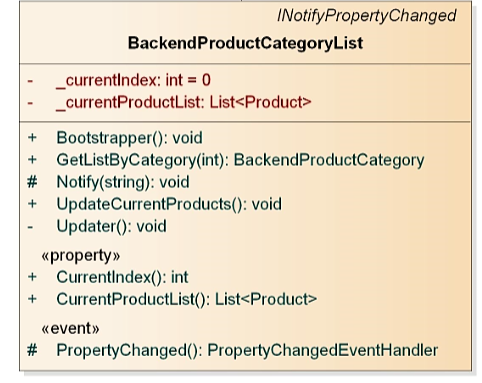
\includegraphics[width=0.30\textwidth]{Systemdesign/backend/klassebeskrivelser/Images/BPCList.png}
    \caption{BackendProductCategoryList}
    \label{fig:BackendProductCategoryList}
\end{figure}
\end{center}
\label{BackendProductCategoryList_Beskrivelse}
 \bigskip 
 
 \textbf{BackendProduct}\\
Denne klasse arver fra \gls{PD} fra \gls{SL}. Klassen implementerer desuden fra INotifyProperyChanged, og derved kan dynamisk opdatere i den grafiske brugerflade. Denne model symboliserer \gls{PD}.
\begin{center}
\begin{figure}[!h]
    \centering
    \includegraphics[width=0.30\textwidth]{Systemdesign/backend/klassebeskrivelser/Images/Backendproduct.png}
    \caption{BackendProduct}
    \label{fig:BackendProduct}
\end{figure}
\end{center}
\label{BackendProduct_Beskrivelse}
 \bigskip 
 
 
  \textbf{ConnectionString}\\
Denne klasse bruges således at der kan fremvises i GUI'en, om der er forbundet til \gls{CS}. Denne implementerer INotifyProperyChanged, således visningen kan opdateres dynamisk.
\begin{center}
\begin{figure}[!h]
    \centering
    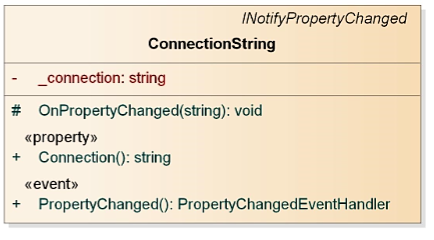
\includegraphics[width=0.30\textwidth]{Systemdesign/backend/klassebeskrivelser/Images/const.png}
    \caption{ConnectionString}
    \label{fig:ConnectionString}
\end{figure}
\end{center}
\label{ConnectionString_Beskrivelse}
 \bigskip 


 \textbf{BackendProductCategory}\\
Denne klasse arver fra \gls{PD} fra \gls{SL}. Klassen implementerer desuden fra INotifyProperyChanged, og derved kan dynamisk opdatere i den grafiske brugerflade. Denne model symboliserer \gls{PDK}.
\begin{center}
\begin{figure}[!h]
    \centering
    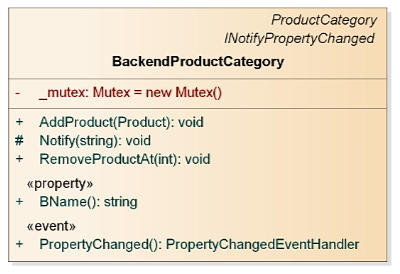
\includegraphics[width=0.30\textwidth]{Systemdesign/backend/klassebeskrivelser/Images/Backendproductcat.png}
    \caption{BackendProductCategory}
    \label{fig:BackendProductCategory}
\end{figure}
\end{center}
\label{BackendProductCategoryr_Beskrivelse}
 \bigskip 

